\documentclass{standalone}
\usepackage{tikz}
\usetikzlibrary{patterns, positioning}
\usepackage[sfdefault]{ClearSans} %% option 'sfdefault' activates Clear Sans as the default text font
\usepackage[T1]{fontenc}

\begin{document}
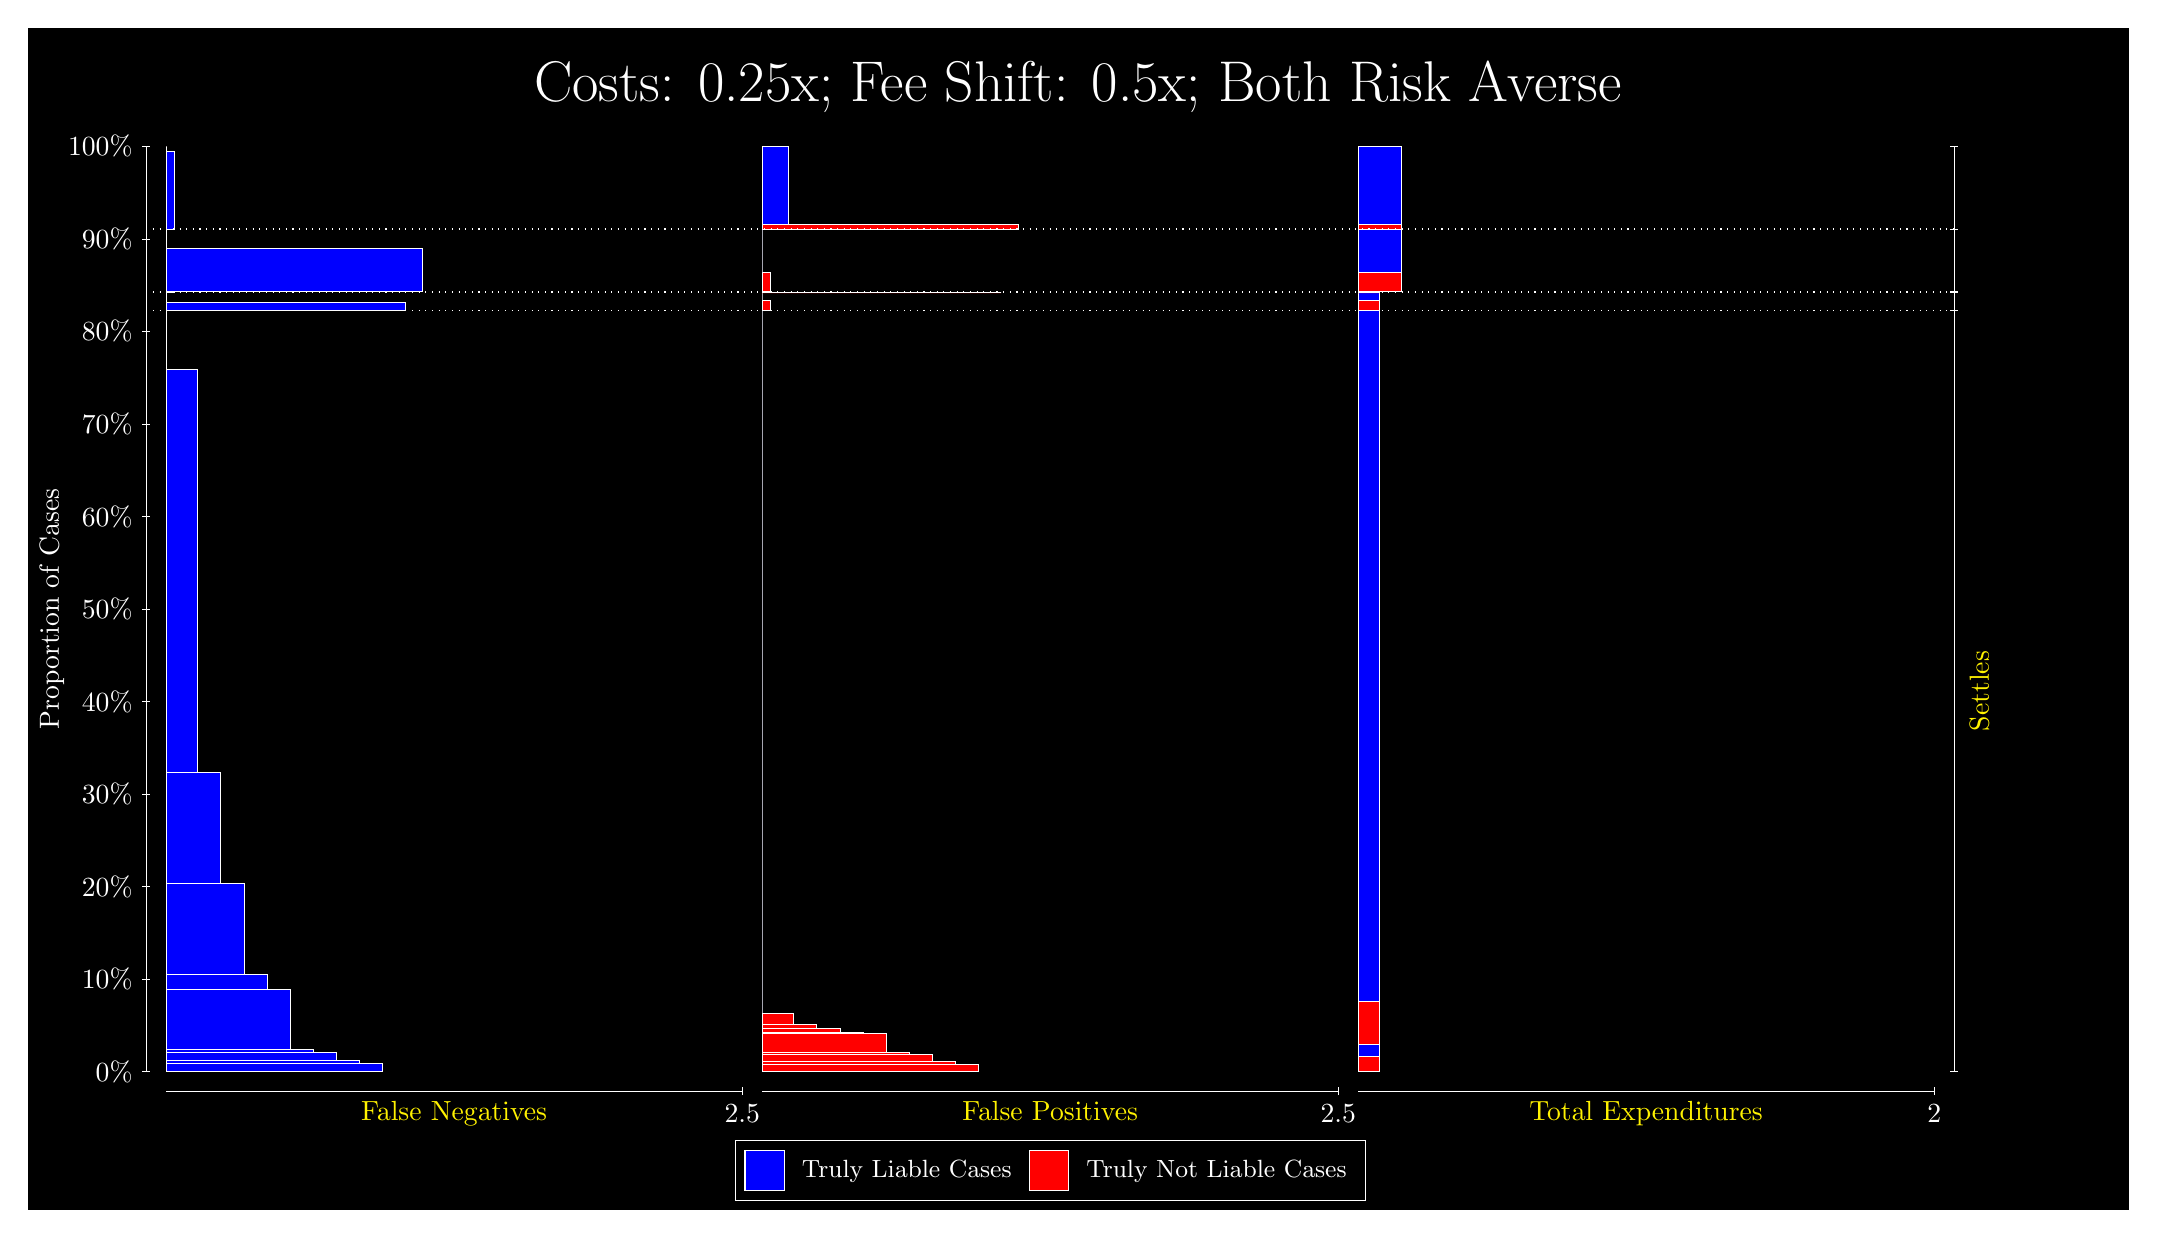
\begin{tikzpicture}
\draw[fill=black] (0,0) rectangle (26.667,15);
\draw[text=white] (0,13.5) rectangle (26.667,15) node[midway] {\huge Costs: 0.25x; Fee Shift: 0.5x; Both Risk Averse};
\draw[white, very thin] (1.5,1.75) -- (1.5,13.5);
\node[rotate=90, text=white, anchor=center] at (0.3, 7.625) {Proportion of Cases};
\draw[white, very thin] (1.45,1.75) -- (1.55,1.75);
\node[text=white, anchor=east] at (1.45, 1.75) {0\%};
\draw[white, very thin] (1.45,2.925) -- (1.55,2.925);
\node[text=white, anchor=east] at (1.45, 2.925) {10\%};
\draw[white, very thin] (1.45,4.1) -- (1.55,4.1);
\node[text=white, anchor=east] at (1.45, 4.1) {20\%};
\draw[white, very thin] (1.45,5.275) -- (1.55,5.275);
\node[text=white, anchor=east] at (1.45, 5.275) {30\%};
\draw[white, very thin] (1.45,6.45) -- (1.55,6.45);
\node[text=white, anchor=east] at (1.45, 6.45) {40\%};
\draw[white, very thin] (1.45,7.625) -- (1.55,7.625);
\node[text=white, anchor=east] at (1.45, 7.625) {50\%};
\draw[white, very thin] (1.45,8.8) -- (1.55,8.8);
\node[text=white, anchor=east] at (1.45, 8.8) {60\%};
\draw[white, very thin] (1.45,9.975) -- (1.55,9.975);
\node[text=white, anchor=east] at (1.45, 9.975) {70\%};
\draw[white, very thin] (1.45,11.15) -- (1.55,11.15);
\node[text=white, anchor=east] at (1.45, 11.15) {80\%};
\draw[white, very thin] (1.45,12.325) -- (1.55,12.325);
\node[text=white, anchor=east] at (1.45, 12.325) {90\%};
\draw[white, very thin] (1.45,13.5) -- (1.55,13.5);
\node[text=white, anchor=east] at (1.45, 13.5) {100\%};

\draw[white, very thin] (24.457,1.75) -- (24.457,13.5);
\draw[white, very thin] (24.407,1.75) -- (24.507,1.75);
\node[anchor=west] at (24.407, 1.75) {};
\draw[white, very thin] (24.407,11.414) -- (24.507,11.414);
\node[anchor=west] at (24.407, 11.414) {};
\draw[white, very thin] (24.407,11.643) -- (24.507,11.643);
\node[anchor=west] at (24.407, 11.643) {};
\draw[white, very thin] (24.407,11.653) -- (24.507,11.653);
\node[anchor=west] at (24.407, 11.653) {};
\draw[white, very thin] (24.407,12.45) -- (24.507,12.45);
\node[anchor=west] at (24.407, 12.45) {};
\draw[white, very thin] (24.407,13.5) -- (24.507,13.5);
\node[anchor=west] at (24.407, 13.5) {};

\draw[white, very thin, fill=blue] (1.75,1.75) rectangle (4.4946,1.8501);
\draw[white, very thin, fill=blue] (1.75,1.8501) rectangle (4.2018,1.8992);
\draw[white, very thin, fill=blue] (1.75,1.8992) rectangle (3.9091,1.9915);
\draw[white, very thin, fill=blue] (1.75,1.9915) rectangle (3.6163,2.0327);
\draw[white, very thin, fill=blue] (1.75,2.0327) rectangle (3.3236,2.7952);
\draw[white, very thin, fill=blue] (1.75,2.7952) rectangle (3.0308,2.9901);
\draw[white, very thin, fill=blue] (1.75,2.9901) rectangle (2.738,4.1418);
\draw[white, very thin, fill=blue] (1.75,4.1418) rectangle (2.4453,5.5506);
\draw[white, very thin, fill=blue] (1.75,5.5506) rectangle (2.1525,10.67);
\draw[white, very thin, fill=red] (1.75,10.67) rectangle (1.75,11.414);
\draw[white, very thin, fill=blue] (1.75,11.414) rectangle (4.7873,11.516);
\draw[white, very thin, fill=red] (1.75,11.516) rectangle (1.75,11.643);
\draw[white, very thin, fill=blue] (1.75,11.643) rectangle (1.8598,11.652);
\draw[white, very thin, fill=red] (1.75,11.652) rectangle (1.75,11.653);
\draw[white, very thin, fill=blue] (1.75,11.653) rectangle (5.0069,12.207);
\draw[white, very thin, fill=red] (1.75,12.207) rectangle (1.75,12.45);
\draw[white, very thin, fill=blue] (1.75,12.45) rectangle (1.8598,13.439);
\draw[white, very thin, fill=red] (1.75,13.439) rectangle (1.75,13.5);
\draw[white, very thin, fill=red] (9.3189,1.75) rectangle (12.063,1.8372);
\draw[white, very thin, fill=red] (9.3189,1.8372) rectangle (11.771,1.8769);
\draw[white, very thin, fill=red] (9.3189,1.8769) rectangle (11.478,1.965);
\draw[white, very thin, fill=red] (9.3189,1.965) rectangle (11.185,1.9923);
\draw[white, very thin, fill=red] (9.3189,1.9923) rectangle (10.892,2.2296);
\draw[white, very thin, fill=red] (9.3189,2.2296) rectangle (10.6,2.2514);
\draw[white, very thin, fill=red] (9.3189,2.2514) rectangle (10.307,2.3003);
\draw[white, very thin, fill=red] (9.3189,2.3003) rectangle (10.014,2.3507);
\draw[white, very thin, fill=red] (9.3189,2.3507) rectangle (9.7214,2.4943);
\draw[white, very thin, fill=blue] (9.3189,2.4943) rectangle (9.3189,11.414);
\draw[white, very thin, fill=red] (9.3189,11.414) rectangle (9.4287,11.542);
\draw[white, very thin, fill=blue] (9.3189,11.542) rectangle (9.3189,11.643);
\draw[white, very thin, fill=red] (9.3189,11.643) rectangle (12.356,11.643);
\draw[white, very thin, fill=blue] (9.3189,11.643) rectangle (9.4287,11.653);
\draw[white, very thin, fill=red] (9.3189,11.653) rectangle (9.4287,11.895);
\draw[white, very thin, fill=blue] (9.3189,11.895) rectangle (9.3189,12.45);
\draw[white, very thin, fill=red] (9.3189,12.45) rectangle (12.576,12.511);
\draw[white, very thin, fill=blue] (9.3189,12.511) rectangle (9.6482,13.5);
\draw[white, very thin, fill=red] (16.888,1.75) rectangle (17.162,1.944);
\draw[white, very thin, fill=blue] (16.888,1.944) rectangle (17.162,2.0932);
\draw[white, very thin, fill=red] (16.888,2.0932) rectangle (17.162,2.6435);
\draw[white, very thin, fill=blue] (16.888,2.6435) rectangle (17.162,11.414);
\draw[white, very thin, fill=red] (16.888,11.414) rectangle (17.162,11.542);
\draw[white, very thin, fill=blue] (16.888,11.542) rectangle (17.162,11.643);
\draw[white, very thin, fill=red] (16.888,11.643) rectangle (17.162,11.643);
\draw[white, very thin, fill=blue] (16.888,11.643) rectangle (17.162,11.653);
\draw[white, very thin, fill=red] (16.888,11.653) rectangle (17.437,11.895);
\draw[white, very thin, fill=blue] (16.888,11.895) rectangle (17.437,12.45);
\draw[white, very thin, fill=red] (16.888,12.45) rectangle (17.437,12.511);
\draw[white, very thin, fill=blue] (16.888,12.511) rectangle (17.437,13.5);
\draw[white, dotted] (1.5,11.414) -- (24.457,11.414);
\draw[white, dotted] (1.5,11.643) -- (24.457,11.643);
\draw[white, dotted] (1.5,11.653) -- (24.457,11.653);
\draw[white, dotted] (1.5,12.45) -- (24.457,12.45);
\draw[white, very thin] (1.75,1.5) -- (9.0689,1.5);
\node[text=yellow, anchor=north] at (5.4094, 1.5) {False Negatives};
\draw[white, very thin] (9.0689,1.45) -- (9.0689,1.55);
\node[text=white, anchor=north] at (9.0689, 1.45) {2.5};

\draw[white, very thin] (9.3189,1.5) -- (16.638,1.5);
\node[text=yellow, anchor=north] at (12.978, 1.5) {False Positives};
\draw[white, very thin] (16.638,1.45) -- (16.638,1.55);
\node[text=white, anchor=north] at (16.638, 1.45) {2.5};

\draw[white, very thin] (16.888,1.5) -- (24.207,1.5);
\node[text=yellow, anchor=north] at (20.547, 1.5) {Total Expenditures};
\draw[white, very thin] (24.207,1.45) -- (24.207,1.55);
\node[text=white, anchor=north] at (24.207, 1.45) {2};

\node[text=yellow, centered, rotate=90] at (24.777, 6.5822) {Settles};





\draw (12.978300999999998,1.5) node[draw=none] (baseCoordinate) {};
\begin{scope}[align=center]
        \matrix[scale=0.5, draw=white, below=0.5cm of baseCoordinate, nodes={draw}, column sep=0.1cm]{
            \node[rectangle, draw, minimum width=0.5cm, minimum height=0.5cm, fill=blue] {}; &
            \node[draw=none, font=\small, text=white] (B) {Truly Liable Cases}; &
            \node[rectangle, draw, minimum width=0.5cm, minimum height=0.5cm, fill=red] {}; &
            \node[draw=none, font=\small, text=white] (B) {Truly Not Liable Cases}; \\
            };
\end{scope}

\end{tikzpicture}
\end{document}